\section{Counterfactual supervision across native
teachers}\label{counterfactual-supervision-across-native-teachers}

\subsection{Reconstruction and causal
domains}\label{reconstruction-and-causal-domains}

We reconstruct M6B from authenticated original source and 21 historical
artifacts. The 249/500 traditional, 476/500 own-proposal and 500/500
counterfactual outcomes concern one training seed, 10001, on paired
cubic N10240 cases. Thirty original-policy executions are replayed
exactly. M6B uses the 8967-parameter M4B architecture, whereas canonical
E1 has 16035 parameters. The own/CF checkpoints share every
participation, first-message and candidate tensor; only the
second-message and COMMIT tensors differ. The configured 120-epoch
horizon is 17760 updates; the selected checkpoints are epoch 53, or 7844
updates. The traditional comparison also changes the number of tapes per
graph, so its improvement is not a pure CF effect.

Pedro's 16 source hashes are verified against commits fc756cef, 80f486eb
and 6836d855. None of the 40 expected original E1 weight hashes was
recovered from 6614 local checkpoint files or the inspected public
release manifests. His five 1980/1980 results, JP 1631/1980 and GM
1951/1980 remain authenticated reported evidence with five
initializations over 396 published cases and a common training pool. His
17760 updates of 1680 roots and own/CF training also differ from the
primary 500-update, batch 64 passive study. New runs below reproduce
mechanisms, not those unavailable original policies.

We define a phase-specific label operation

\[\mathcal O_T(S,a,\xi)=D_T^\phi\bigl(R_T^\phi(S,a,\xi)\bigr),\]

where \(S\) is an admissible native snapshot, \(a\) a typed
intervention, \(\xi\) the private input, and \(R\) recomputes every
causal descendant before the phase decision \(D\) is queried. We
distinguish native decisions from defensive continuation queries on
offers that the native policy might not emit. The latter are additional
supervised tasks, not a claim that arbitrary simulator arrays are
reachable teacher states. For BE and JP, forced participation cannot
bypass phase eligibility or priority; ColorTrials confirmation requires
strict winning preferences under actual availability. Linial points and
GM detection marks have separate native oracles.

Admissible contexts are reconstructed from legal prefixes. Changing IDs
requires a new complete replay, including comparisons, blocks,
permissions and auxiliary initial colors. Private preference/draw
interventions preserve the persistent state and regenerate messages. KW
arithmetic and Linial evaluations are recomputed; speculative GM
histories retain their supplied schedule, actual assignment colors,
marks and repair queue. We export 162 additional hard contexts with
replay witnesses. The three palette cores share these training-only
adapters. All teacher and autonomous inference source files remain
unchanged from the baseline; no exact decision replaces the neural
confirmation head.

\subsection{Paired controls and strict new
certifications}\label{paired-controls-and-strict-new-certifications}

We train 135 primary runs: three pending teachers, three cores, five new
seeds and three treatments. Each preserves 500/1500/4000 checkpoints,
the same native bank, initialization and minibatch sequence within a
seed/core. Passive is the historical loss. Matched evaluates COMMIT with
its stored teacher proposals and corresponding label. Fixed-bank CF uses
100 matched warmup updates, then P + C + .5 matched confirmation + .5 CF
confirmation. Each normal root acquires three native component labels
and four additional stored confirmation queries; Linial and DETECT each
acquire one native label. Own-proposal queries in a separate
seven-teacher pilot are charged individually.

Training uses N8/12/16/24. An amendment recorded before the additional
screen and all new finals expands development from 60 to 300 cases at
N28/36. The first common perfect checkpoint is frozen per treatment.
Final has five independent 1000-case batteries at N32/48/64, ten fixed
family strata, native horizons, and the strict original
invariant/terminal gate.

Matched passes all nine pending packages, using 1500 updates for BE, 500
for ColorTrials/E1, 1500 for its other cores and 500 for GM. CF
initially fails BE at 1500 in seed 94105 for all cores, and
ColorTrials/E1 at 500 in seed 94103. Independently frozen follow-ups
compare existing 1500/4000 CF checkpoints on new namespaces, retaining
both outcomes. BE 1500 again fails in seed 94105;
ColorTrials/Transformer1500 has two failures in its new battery. All six
4000-update packages pass. The following CF fixed points therefore close
all nine cells, while the historical twelve remain separate: coverage is
21/21, not one homogeneous newly retrained cohort.

{\def\LTcaptype{none} % do not increment counter
\begin{longtable}[]{@{}llllll@{}}
\toprule\noalign{}
Teacher & Core & Updates & Native labels & All labels & Final \\
\midrule\noalign{}
\endhead
\bottomrule\noalign{}
\endlastfoot
BE & normalized & 4000 & 3000 & 6776 & 5 x 1000/1000 \\
BE & deepsets & 4000 & 3000 & 6776 & 5 x 1000/1000 \\
BE & transformer & 4000 & 3000 & 6776 & 5 x 1000/1000 \\
ColorTrials & normalized & 4000 & 30000 & 70000 & 5 x 1000/1000 \\
ColorTrials & deepsets & 4000 & 30000 & 70000 & 5 x 1000/1000 \\
ColorTrials & transformer & 4000 & 30000 & 70000 & 5 x 1000/1000 \\
GM & normalized & 500 & 3000 & 6104--6120 & 5 x 1000/1000 \\
GM & deepsets & 500 & 3000 & 6104--6120 & 5 x 1000/1000 \\
GM & transformer & 500 & 3000 & 6104--6120 & 5 x 1000/1000 \\
\end{longtable}
}

The complete extension retains 195000 final execution rows, 194979
correct, and 170 distinct frozen checkpoints. Repeated checkpoints on a
second battery are not new training replicas. All eight representative
failed checkpoint/battery traces reproduce their original outcomes under
the same 32-case cohort and 1024-root numerical batching. BE failures
are omitted required KW recolorings that violate the new auxiliary
bound. No failure is repaired or removed. An explicit erratum preserves
and corrects the CT follow-up plan's reason-text typo (the original E1
failure was at 500, not1500); the actual checkpoint hashes, batteries
and rows are unchanged.

\begin{figure}
\centering
\pandocbounded{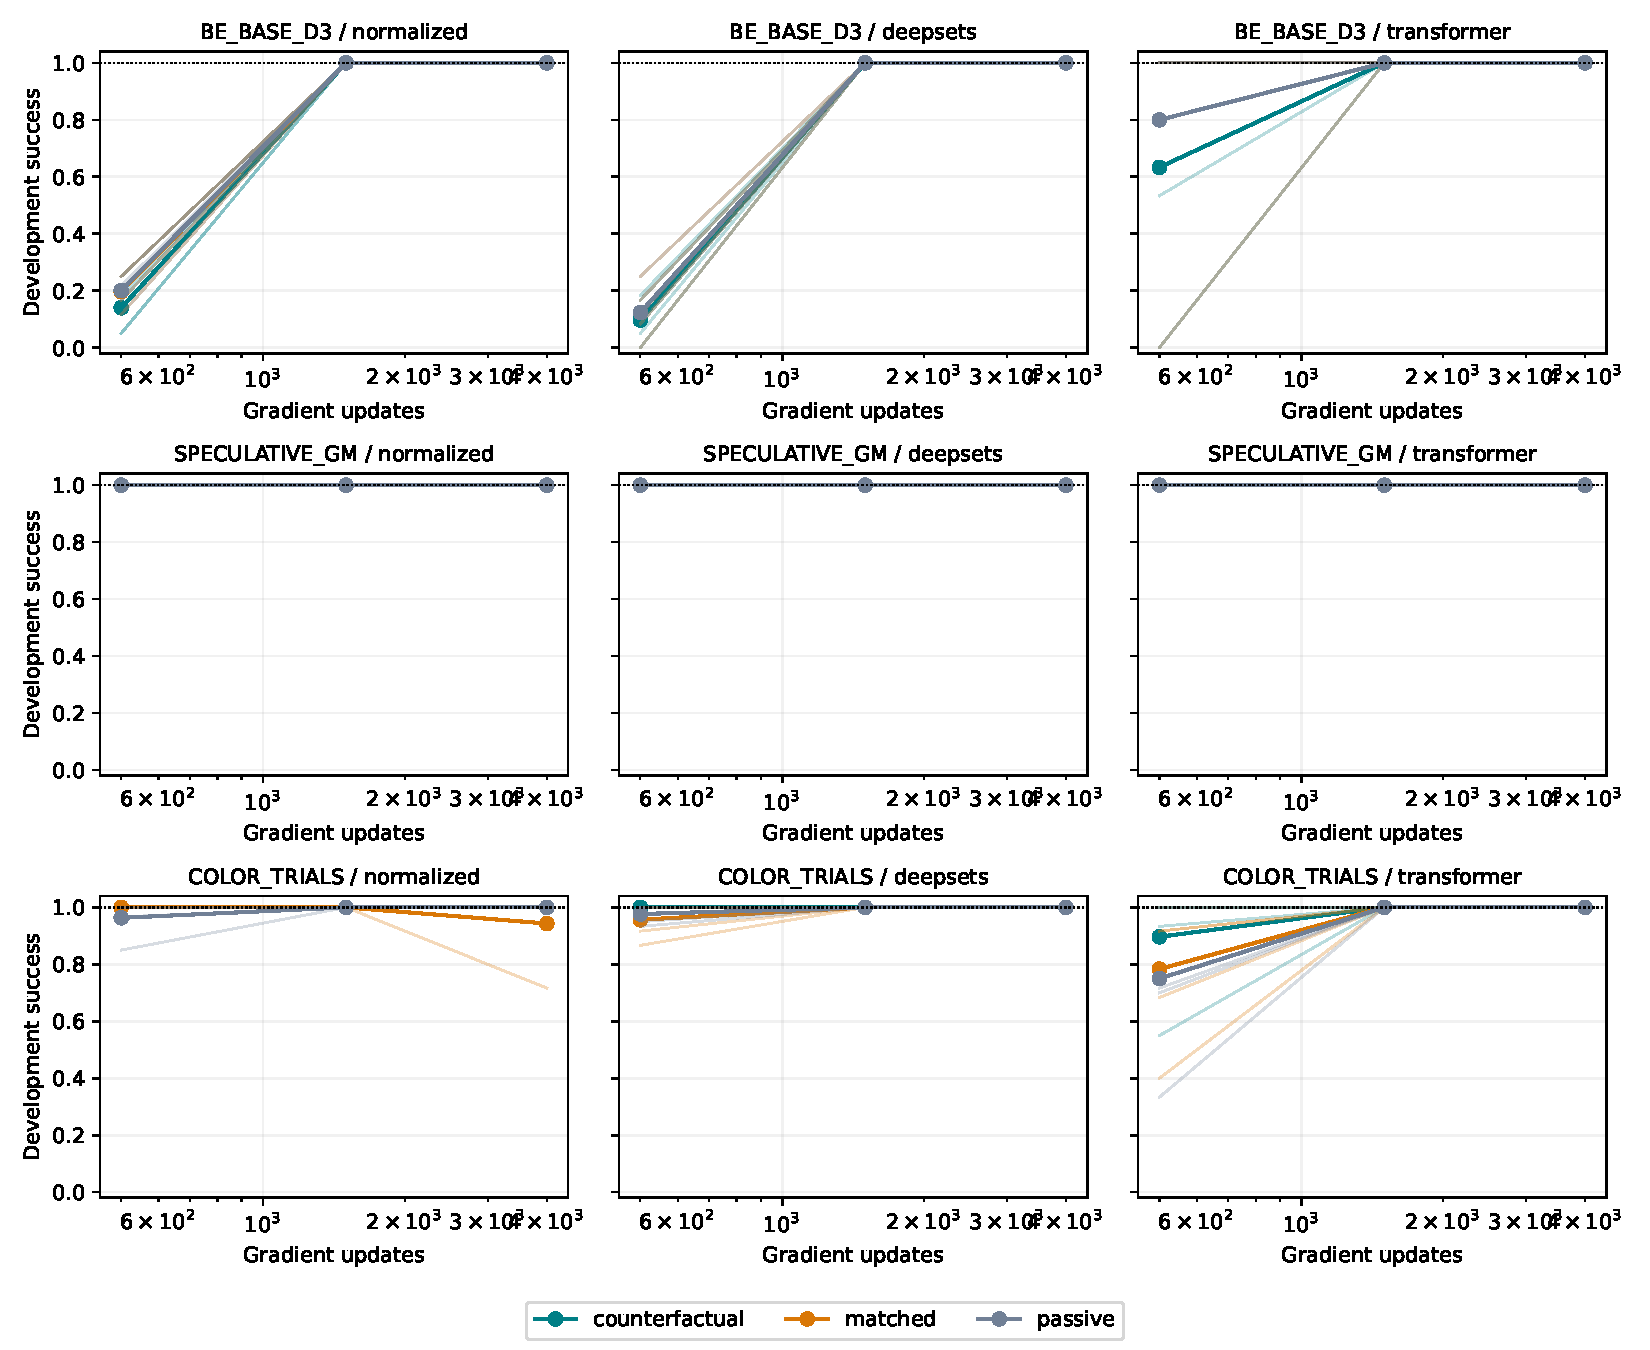
\includegraphics[keepaspectratio,alt={All five unsmoothed development curves and descriptive means at fixed native banks. Perfect development is a selection screen, not a functional certificate.}]{figures/multicf-optimization-curves.pdf}}
\caption{All five unsmoothed development curves and descriptive means at
fixed native banks. Perfect development is a selection screen, not a
functional certificate.}
\end{figure}

\subsection{Functional validity and continuation
fidelity}\label{functional-validity-and-continuation-fidelity}

At 4000, all permitted roots in 60 common native development
trajectories per seed are audited, with four fresh continuation queries
per color root. The table reports descriptive aggregate percentages
across five policies; root decisions are not independent training
replicas. Per core, the CF denominators are 499200 for BE, 41036 for GM
and 57576 for ColorTrials. Full per-seed action, actual-transition,
component and phase counts remain machine-readable. The certified GM500
policies have separate full audits at their actual checkpoint; the table
fixes4000 for the paired comparison. CF improves the broader
continuation task, while the matched/passive procedures already satisfy
the functional gate. Thus CF is not uniformly necessary, or better at
the same update count, for native functional success. A matched
ColorTrials/E1 run regresses from 60/60 to 43/60 development successes
between 1500 and4000 updates.

{\def\LTcaptype{none} % do not increment counter
\begin{longtable}[]{@{}
  >{\raggedright\arraybackslash}p{(\linewidth - 8\tabcolsep) * \real{0.2000}}
  >{\raggedright\arraybackslash}p{(\linewidth - 8\tabcolsep) * \real{0.2000}}
  >{\raggedright\arraybackslash}p{(\linewidth - 8\tabcolsep) * \real{0.2000}}
  >{\raggedright\arraybackslash}p{(\linewidth - 8\tabcolsep) * \real{0.2000}}
  >{\raggedright\arraybackslash}p{(\linewidth - 8\tabcolsep) * \real{0.2000}}@{}}
\toprule\noalign{}
\begin{minipage}[b]{\linewidth}\raggedright
Teacher
\end{minipage} & \begin{minipage}[b]{\linewidth}\raggedright
Core
\end{minipage} & \begin{minipage}[b]{\linewidth}\raggedright
Matched CF (\%)
\end{minipage} & \begin{minipage}[b]{\linewidth}\raggedright
CF-trained CF (\%)
\end{minipage} & \begin{minipage}[b]{\linewidth}\raggedright
CF native actions (\%)
\end{minipage} \\
\midrule\noalign{}
\endhead
\bottomrule\noalign{}
\endlastfoot
BE & normalized & 9.269 & 99.993 & 100.000 \\
BE & deepsets & 9.269 & 99.993 & 100.000 \\
BE & transformer & 9.269 & 99.993 & 100.000 \\
GM & normalized & 75.363 & 100.000 & 100.000 \\
GM & deepsets & 75.363 & 100.000 & 100.000 \\
GM & transformer & 75.363 & 100.000 & 99.995 \\
ColorTrials & normalized & 97.256 & 99.745 & 99.187 \\
ColorTrials & deepsets & 99.097 & 100.000 & 100.000 \\
ColorTrials & transformer & 98.076 & 100.000 & 100.000 \\
\end{longtable}
}

For BE/GM, every second-stage and COMMIT tensor is identical across the
three palette cores in each paired fixed-proposal seed/update
comparison. Those losses do not use the candidate scorer, whereas
ColorTrials reads its candidate after the second exchange and couples
those gradients. Shared heads explain correlated architecture outcomes;
they do not provide three independent confirmations of a head-level
effect.

\begin{figure}
\centering
\pandocbounded{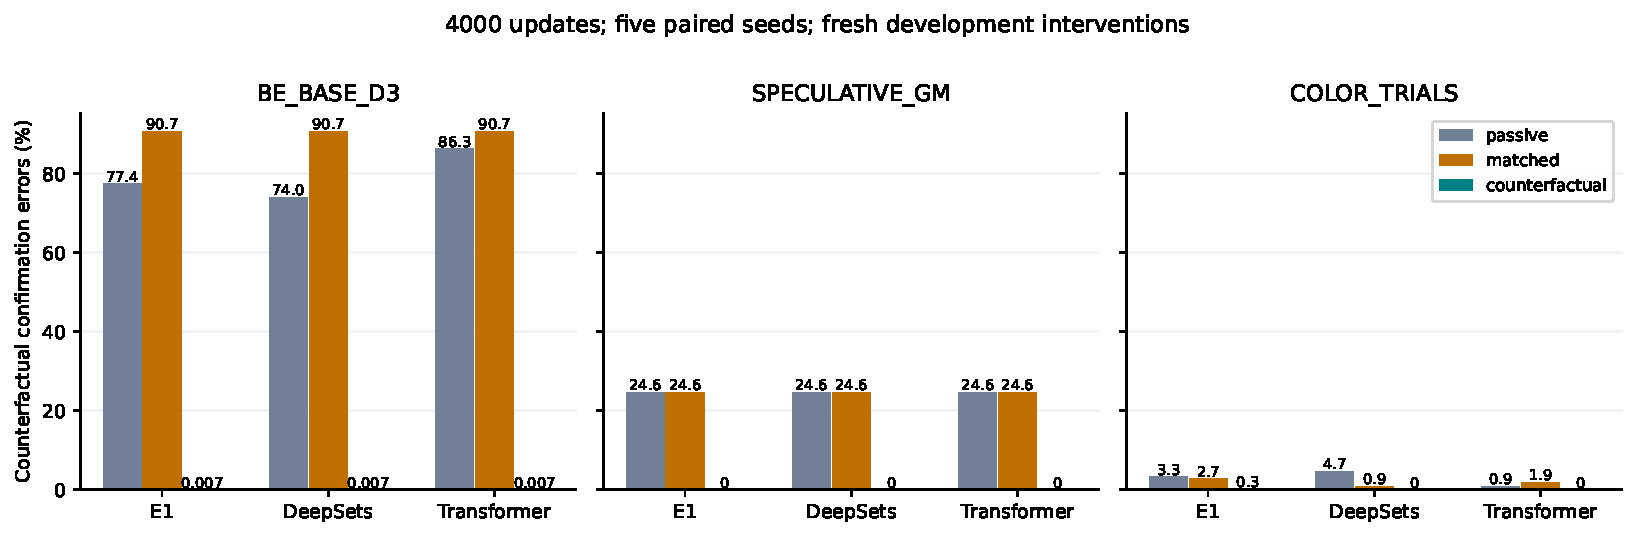
\includegraphics[keepaspectratio,alt={Errors on fresh continuation queries, separated from native action fidelity. Small nonzero errors retain explicit labels.}]{figures/multicf-counterfactual-fidelity.pdf}}
\caption{Errors on fresh continuation queries, separated from native
action fidelity. Small nonzero errors retain explicit labels.}
\end{figure}

Nested ColorTrials banks at native budgets 1000/3000/10000/30000 and
fixed 500/1500 updates provide development-only supervision curves.
Every CF label is charged; these do not establish a new certified
minimum. A matched GM control without the added isolate families also
passes all five new development seeds, so the tested ablation does not
isolate a positive coverage effect. The authenticated old seed 83105
failures and all 30 new regressions remain a separate observation. The
own-plus-CF portability pilot passes 60/60 development in six teachers
for one new E1 seed, but BE obtains 22/60 at 1500; copying the Luby
curriculum is insufficient evidence of a uniformly successful
multiteacher procedure.

\begin{figure}
\centering
\pandocbounded{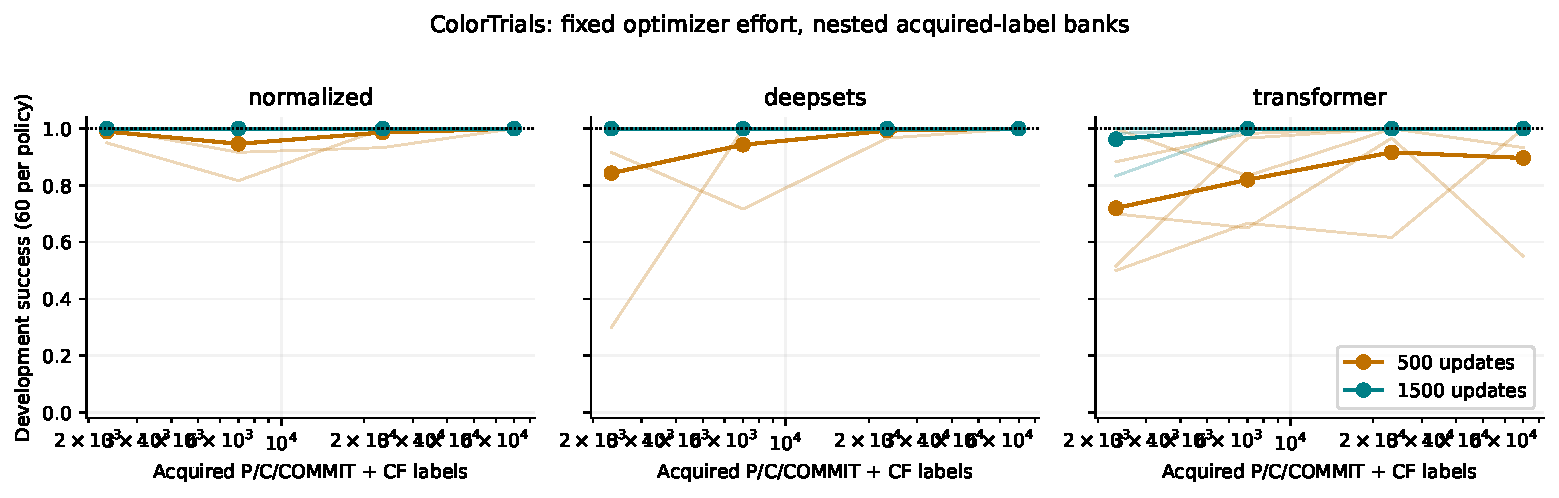
\includegraphics[keepaspectratio,alt={Supervision and optimization are distinct axes; thin lines show all five seeds. These lower-budget points have no new final certification.}]{figures/multicf-supervision-curves.pdf}}
\caption{Supervision and optimization are distinct axes; thin lines show
all five seeds. These lower-budget points have no new final
certification.}
\end{figure}

\subsection{Information, complete outputs and
transfer}\label{information-complete-outputs-and-transfer}

JP's information control fixes the architecture, labels, batches, 500
updates and initialization, changing only two local context channels.
Relative order passes all five 60-case development suites; raw endpoint
IDs, differences and removed IDs do not. Twenty numerical replays
reproduce every original ablation weight tensor and retain intermediate
Adam/RNG checkpoints.

{\def\LTcaptype{none} % do not increment counter
\begin{longtable}[]{@{}ll@{}}
\toprule\noalign{}
JP representation & Development successes, five seeds (/60) \\
\midrule\noalign{}
\endhead
\bottomrule\noalign{}
\endlastfoot
without\_ids & 6, 6, 6, 6, 6 \\
numeric\_ids & 13, 11, 6, 26, 15 \\
numeric\_differences & 16, 15, 19, 31, 20 \\
relative\_comparisons & 60, 60, 60, 60, 60 \\
\end{longtable}
}

An indistinguishability witness swaps the IDs on a pending edge:
anonymous observations are equal but native eligibility reverses. Edge
order suffices for the implemented priority decision. This is an
observation-level obstruction, not a claim that numeric IDs are
unlearnable. ColorTrials has a second-hop availability witness.
Historical M6 also aliases the float64 draws \(1/2-2^{-28}\) and
\(1/2+2^{-28}\) to the same float32 observation, despite opposite
activation labels. The current native teacher directly queries its
supplied float32 inputs, avoiding that particular obstruction.

\begin{figure}
\centering
\pandocbounded{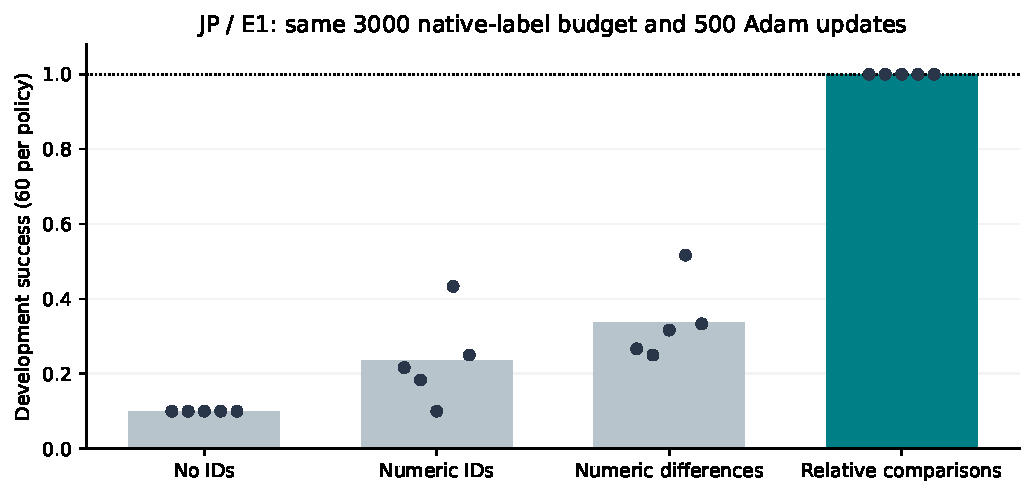
\includegraphics[keepaspectratio,alt={Information representation at a fixed optimizer and label point. Each dot is one training seed; development performance is not final certification.}]{figures/multicf-jp-information.pdf}}
\caption{Information representation at a fixed optimizer and label
point. Each dot is one training seed; development performance is not
final certification.}
\end{figure}

After functional selection, all 45 successful CF policies are frozen
before fresh law and transfer tapes. On path8 and K4 plus four isolates,
256 shared-input runs per graph/policy compare the full labelled
terminal vector and status, without success filtering. The coupling
inequality and exact one-sided binomial bounds with Bonferroni .05/90
yield 89/90 simultaneous TV-at-most-.05 certificates. These are
approximate fixed-graph marginal-law bounds, not equality.
ColorTrials/E1 seed 94104 on path8 has36/256 coupled disagreements,
upper bound .223630 and mean 2.191406 native steps versus 2.097656.
Coupled disagreement is not a TV lower bound or proof that the marginal
laws differ. Empirical full-vector histograms and native times are
retained separately.

Exploratory transfer obtains 3780/3780 correct executions, 84 per policy
at N128/256/512. Its ten domain families are supplemented by binary
trees, diamond chains, triangle chains and subdivided K4 components, all
of maximum degree3. These finite observations do not extend the teacher
to higher degree, local palettes or arbitrary graphs/tapes. Functional
validity does not establish universal decision or law identity.

The complete campaign contains 278 computational training runs,
including paired arms, pilots and numerical replays, with 683504
gradient updates and 2.580 CPU optimization hours. Training GPU time is
zero; the original M6 CUDA replay is separate. Process times overlap.
Acquired components, reused labels, presentations, simulator work and
optimization remain separate; no sample-efficiency claim compares
unequal update budgets. All sources, models, datasets, witnesses,
negative results and manifests accompany this extension. The
verification recomputes every final gate and all stored CF labels with
zero label inconsistencies. The full suite's639 cases and29 later added
cases pass.

These contributions complement trace-oriented CLRS
\citet{velickovic2022clrs} and learner-state acquisition in DAgger
\citet{ross2011dagger}. Recent contrastive graph-coloring work
\citet{le2026contrastive} studies approximate-coloring objectives. Our
contribution is the specified admissible-oracle framework, controlled
separation of training factors, and finite native execution evidence; no
comprehensive bibliographic priority or universal learnability claim
follows from this study.
